\chapter{Proposed Approach}
\label{chap:Chapter4}
%-------------------------------------------------------------------------------%

\section{Concept}
Fixed-pitch proprotor (FPP) system limitations can be addressed by developing variable-pitch proprotors.
Adjusting the pitch in both flight phases may be more complex and expensive but it offers more adaptability and a great positive impact on the overall propulsion system efficiency, increasing the endurance and range.
The \gls{uav} will consume less in hover and the cruise speed will be much higher.\\

This way, the proposed solution for this problem is to develop a stand-alone variable-pitch proprotor system that can, in real-time, change the propeller pitch according to each flight phase.

%-------------------------------------------------------------------------------%

\section{Requirements}
It is important to define requirements, for this system, to better understand the fixed-pitch propeller's limitations and to develop the necessary functionalities to achieve a variable-pitch proprotor system.\\
This way, the requirements should align with mechanical, control, communication, integration, and validation specifications.

\begin{itemize}
    \item \textbf{Mechanical Requirements}
          \begin{enumerate}[start=1,label={\upshape\bfseries (REQ\_0\arabic*):},wide = 0pt, leftmargin = 3em]
              \item The system shall be designed to retrofit existing \glspl{uav} or integrate seamlessly into new \gls{uav} designs.
              \item The variable-pitch mechanism shall be lightweight to minimize the impact on overall \gls{uav} weight and balance.
              \item The system shall be able to withstand the operational stresses and environmental conditions encountered during \gls{uav} flights.
          \end{enumerate}

    \item \textbf{Control System Requirements}
          \begin{enumerate}[start=04,label={\bfseries (REQ\_0\arabic*):},wide = 0pt, leftmargin = 3em]
              \item The control system shall enable real-time adjustment of the proprotor pitch during different flight phases.
              \item It shall incorporate failsafe mechanisms to respond to unexpected malfunctions or loss of communication and revert to a fixed-pitch state in case of critical failures.
              \item The system shall provide precise control over the pitch angle, allowing for fine adjustments to optimize performance.
          \end{enumerate}

    \item \textbf{Wireless Communication Requirements}
          \begin{enumerate}[start=07,label={\bfseries (REQ\_0\arabic*):},wide = 0pt, leftmargin = 3em]
              \item The wireless communication system shall be reliable, with minimal latency to ensure quick response times.
              \item It shall operate within designated frequency bands and comply with relevant aviation communication standards.
              \item Security measures shall be implemented to prevent unauthorized access or interference with the control signals.
          \end{enumerate}

    \item \textbf{Integration Requirements}
          \begin{enumerate}[start=10,label={\bfseries (REQ\_\arabic*):},wide = 0pt, leftmargin = 3em]
              \item The system shall be designed for easy integration with common \gls{uav} autopilot systems.
              \item It shall have compatibility with existing \gls{uav} avionics and navigation systems.
              \item The variable-pitch system shall not interfere with other onboard sensors or communication systems.
          \end{enumerate}

    \item \textbf{Testing and Validation Requirements}
          \begin{enumerate}[start=13,label={\bfseries (REQ\_\arabic*):},wide = 0pt, leftmargin = 3em]
              \item The system shall undergo rigorous testing under various operational scenarios, including weather conditions and flight profiles.
              \item Validation shall include simulated and real-world flights to assess performance and reliability.
              \item The system shall comply with relevant aviation regulations and standards.
          \end{enumerate}
\end{itemize}
%-------------------------------------------------------------------------------%

\section{System Architecture}
As it is possible to see, in the proposed implementation of the System Architecture diagram (figure \ref{fig:system_diagram}), the system will be composed of two subsystems: the Main Device Unit (MDU) and (multiple) Secondary Device Unit (SDU).

\begin{figure}[H]
    \centering
    %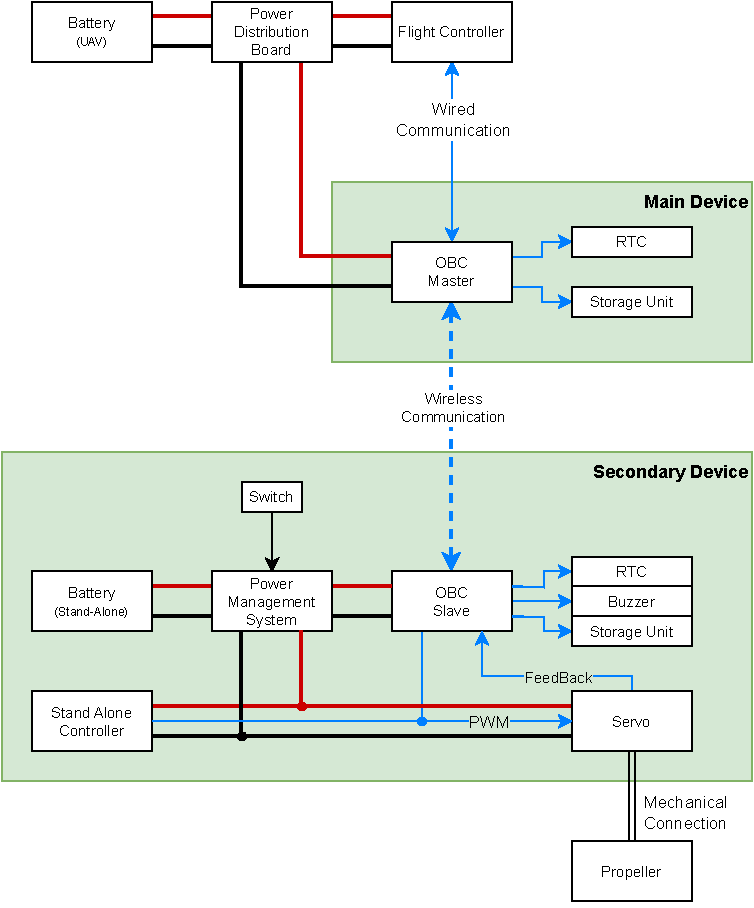
\includegraphics[width=\textwidth,keepaspectratio]{ch3/assets/system_diagram.pdf}
    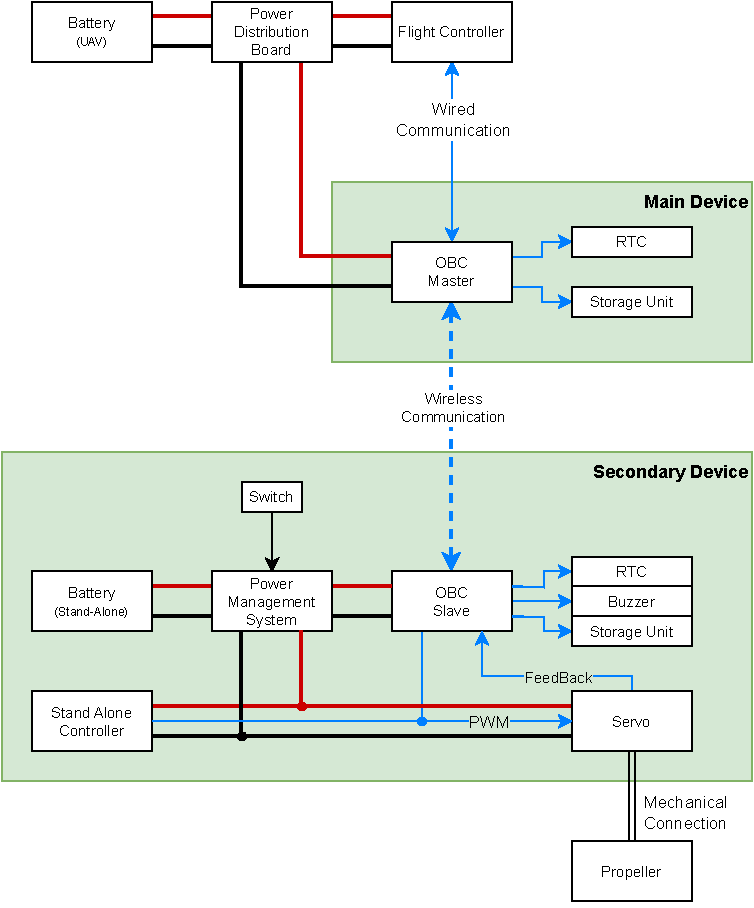
\includegraphics[scale=1]{ch3/assets/system_diagram.pdf}
    \caption{Proposed System Architecture High Level Diagram}
    \label{fig:system_diagram}
\end{figure}

The subsystems can be consider as stand-alone since the main \gls{uav} can work without the subsystems.
These subsystems, described in the next subchapters, are responsible for monitoring the flight phase and control the propeller pitch angle.

\subsection{Main Device}
This subsystem will be, mainly, composed by an \gls{OBC}, a \gls{RTC}, a Storage Unit, and a wireless communication module.\\
The MDU will communicate with the Flight Controller and the SDUs by receiving and transmitting information.

With the Flight Controller, through wired communication, the MDU will:
\begin{itemize}
    \item Receive
          \begin{itemize}
              \item Flight Phase message
              \item Maneuver control message
              \item \gls{GNSS} epoch time
              \item Heartbeat signal
          \end{itemize}
    \item Transmit
          \begin{itemize}
              \item Heartbeat signal
              \item System Status message
          \end{itemize}
\end{itemize}

The Flight Phase message and the Maneuver Control message will inform the MDU about the current flight phase and the need to make additional adjustments to the propeller pitch.
After interpreting the message, the \gls{OBC} will send a control command. This control command will be explained further in this chapter\\

The \gls{GNSS} epoch time will update the \gls{OBC} date and time (periodically or on startup). With the help of the \gls{RTC}, the MDU system will be able to maintain the date and time even when the \gls{uav} system is powered off.
The \gls{GNSS} epoch time will be helpful when storing system logs (in the Storage Unit) and will help to calculate the latency of the communication between devices.\\

Lastly, the received heartbeat signal will work as a \textit{keep alive} mechanism informing, this way, the \gls{OBC} if the system is powered on.
This will help save power since the \gls{OBC} can shut down when the Flight Controller turns off.\\

The transmitted heartbeat, which also works as a \textit{keep alive} mechanism, will inform the Flight Controller that the MDU is working correctly.
This function will be crucial because if the MDU is not working (powered off or unresponsive) the \gls{uav} system will need to enter a failsafe mode and land, as soon as possible, since it can no longer control the pitch of the blades.\\

Since the MDU is responsible for managing all the SDUs, it must, periodically, inform the Flight Controller about the overall status of the system, so that, in case of any failure, the Flight Controller may enter in failsafe.\\

With the SDUs, through wireless communication, the MDU will:
\begin{itemize}
    \item Receive
          \begin{itemize}
              \item Heartbeat signal
              \item SDU Status message
          \end{itemize}
    \item Transmit
          \begin{itemize}
              \item Heartbeat signal
              \item Control Command
              \item Epoch Time
          \end{itemize}
\end{itemize}

The received and transmitted heartbeat signals will have the same functionality as explained previously. The MDU and SDUs will inform each other if they are working correctly.\\

The SDU Status message will help the MDU keep track of the status of all Secondary devices. In case of malfunction or if one or more SDUs can't change the propeller pitch, the MDU must be noticed so that it can communicate to the Flight Controller about the failure.\\

The MDU will send a Control Command, containing the desired pitch, to all the SDUs according to the phase of flight message received previously.\\

By sending the epoch time to all the SDUs, it is possible to keep the whole system updated and with the same date and time reference.\\

\subsection{Secondary Device}
This subsystem will be, composed of an \gls{OBC}, a \gls{RTC}, a Storage Unit, a battery (with a power management system), an on/off switch, a buzzer, a stand-alone \gls{PWM} controller, a servo, and a wireless communication module.\\

The on/off switch and the buzzer will work as human-machine interfaces to help the user interact with the system.\\
Since the SDU will be designed to be stand-alone (with a dedicated power supply) the system needs to be powered on manually and the buzzer can notice the user that the system is powering on.\\

The servo, mechanically connected to the propeller, will be responsible for changing the propeller pitch according to the state of flight.
It will be equipped with feedback functionality so that the system can control, more precisely, the pitch and know if the propeller has reached its goal.\\

There will also be implemented a stand-alone \gls{PWM} controller, able to generate a fixed \gls{PWM} signal, to control the servo in case of failure from the \gls{OBC}.
As a failsafe mechanism, if one or more SDUs fail, the \gls{PWM} controller will generate a \gls{PWM} signal fixing the pitch of the propellers to a designated angle.\\
This action will transform the \gls{uav} system into a fixed-pitch proprotor but will help avoid having a system with a single point of failure that can cause the \gls{uav} to crash and possibly hurt people.\\

The Power Management System will be responsible for monitoring the \gls{SoC} of the battery, for converting the voltage from the battery to the needed voltage levels and for distributing to all components.\\
An \gls{UVP} will be also implemented to ensure that the SDU subsystem shutdowns when the battery is at a critical level.


%-------------------------------------------------------------------------------%
\section{System Behavior}

In order to properly design the system behavior it was developed a system flow chart.
The flow chart, represented in figure \ref{fig:MDU_MAIN}, describes the expected high level behavior of both MDU and SDU.
 
\begin{figure}[H]
    \centering
    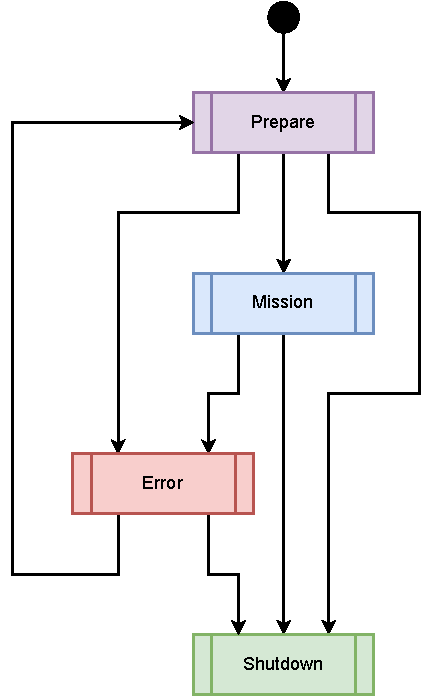
\includegraphics[scale=0.8]{ch3/assets/MDU_MAIN.pdf}
    \caption{Proposed System Behavior - High Level Flow Chart}
    \label{fig:MDU_MAIN}
\end{figure}

In this flow chart, there are four main tasks:
\begin{itemize}
    \item Prepare
    \item Mission
    \item Error
    \item Shutdown
\end{itemize}

\subsection{Main Device Unit Behavior}
In this chapter it is described all the tasks referring to the Main Device Unit Behavior.
\subsubsection{Prepare Task}
The \textbf{Prepare} task is responsible for preparing the subsystem after activation anc checking if the system is ready for mission.

Firstly it will check the connection and the number of  SDUs (this also represents the number of proprotors).
In case of insufficient number of SDUs, the subsystem will enter in a state of Error and enter the \textbf{ERROR} task.

After this the subsystem checks the connection with Flight Controller (FC).
If there is no response from the FC (meaning, for example, that the FC is turned off), the MDU subsystem will turn off by entering in the task \textbf{Shutdown}.

The next step is publish an heartbeat to the SDUs (using topic \textit{mdu\slash  heartbeat}) and to acquire Epoch time to update its own date and time (if not possible use stored date and time) and update all the connected SDUs by publishing in \textit{mdu\slash date\_time} topic.

Finally, in this task, the MDU will subscribe to \textit{sdu\slash heartbeat} and \textit{sdu\slash status}.
If all the SDUs are ready, the subsystem is ready for the mission and, in this case, enter \textbf{Mission} task.
Otherwise, if any or all the SDUs have any problem or can not be reached, the MDU will enter the \textbf{ERROR} task.

The MDU \textbf{Prepare} task flow is represented in figure \ref{fig:MDU_PREPARE} in Appendix \ref{AppendixA}.

\subsubsection{Mission Task}
In the \textbf{Mission} task the MDU will monitor the flight phase (given by the FC) and publish, accordingly, to \textit{mdu\slash pitch\_cmd} topic.
Since each phase requires a different pitch angle, it was defined three flight phases:
\begin{itemize}
    \item Take-Off
    \item Landing
    \item Forward Flight
\end{itemize}
And while Take-Off and Landing phase, the pitch angles are defined, fixed and equal between all proprotors, in Forward Flight phase each maneuver will require a different pitch angle and may require different pitches between each proprotor.

In parallel, the subsystem will also be publishing an heartbeat to the SDUs, check the heartbeat from th FC and monitoring the heartbeat and status of all SDUs.
By constantly monitoring the heartbeat and status of all the SDUs it is possible to recognize errors in the system and try to find solutions (in \textbf{Error} task) to avoid mission failures.

The MDU \textbf{Mission} task flow is represented in figure \ref{fig:MDU_MISSION} in Appendix \ref{AppendixB}\\

\subsubsection{Error Task}
\textbf{Error} task will be responsible for analyzing the error type and try to resolve the error before mission failure.

The MDU Error task flow is represented in figure \ref{fig:MDU_ERROR} in Appendix \ref{AppendixC}\\

\subsubsection{Shutdown Task}
The MDU Shutdown task flow is represented in figure \ref{fig:MDU_SHUTDOWN} in Appendix \ref{AppendixD}\\

\subsection{Secondary Device Unit Behavior}
In the same way, this chapter will describe all the tasks referring to the Secondary Device Unit Behavior.

\subsubsection{Prepare Task}
The SDU Prepare task flow is represented in figure \ref{fig:SDU_PREPARE} in Appendix \ref{AppendixE}\\

\subsubsection{Mission Task}
The SDU Mission task flow is represented in figure \ref{fig:SDU_MISSION} in Appendix \ref{AppendixF}\\

\subsubsection{Error Task}
The SDU Error task flow is represented in figure \ref{fig:SDU_ERROR} in Appendix \ref{AppendixG}\\

\subsubsection{Shutdown Task}
The SDU Shutdown task flow is represented in figure \ref{fig:SDU_SHUTDOWN} in Appendix \ref{AppendixH}\\
%-------------------------------------------------------------------------------%

TODO: CHANGE "TOPICS" TO "NODES" ??
TODO: MORE INFO